\documentclass{article}

% Packages
\usepackage{fullpage}
\usepackage{graphicx}

% Macros

\newcommand{\HWNUM}{1}

\begin{document}

    % TITLE SECTION

    \begin{center}
        ************************************ \\
        EE/CS 119A Homework \HWNUM \\
        Edward Speer \\
        \today \\
        ************************************
    \end{center}

    % PROBLEMS
    \begin{enumerate}
    
        \item \textbf{Problem 1}: \emph{Simple Circuit} \\
        
            From the problem description, either $B$ or $C$ must be inactive
            with $A$ active for $X$ to be active. Clearly, this means that
            $X = A(B' + C')$.

            Active high circuit:
            \begin{center} 
                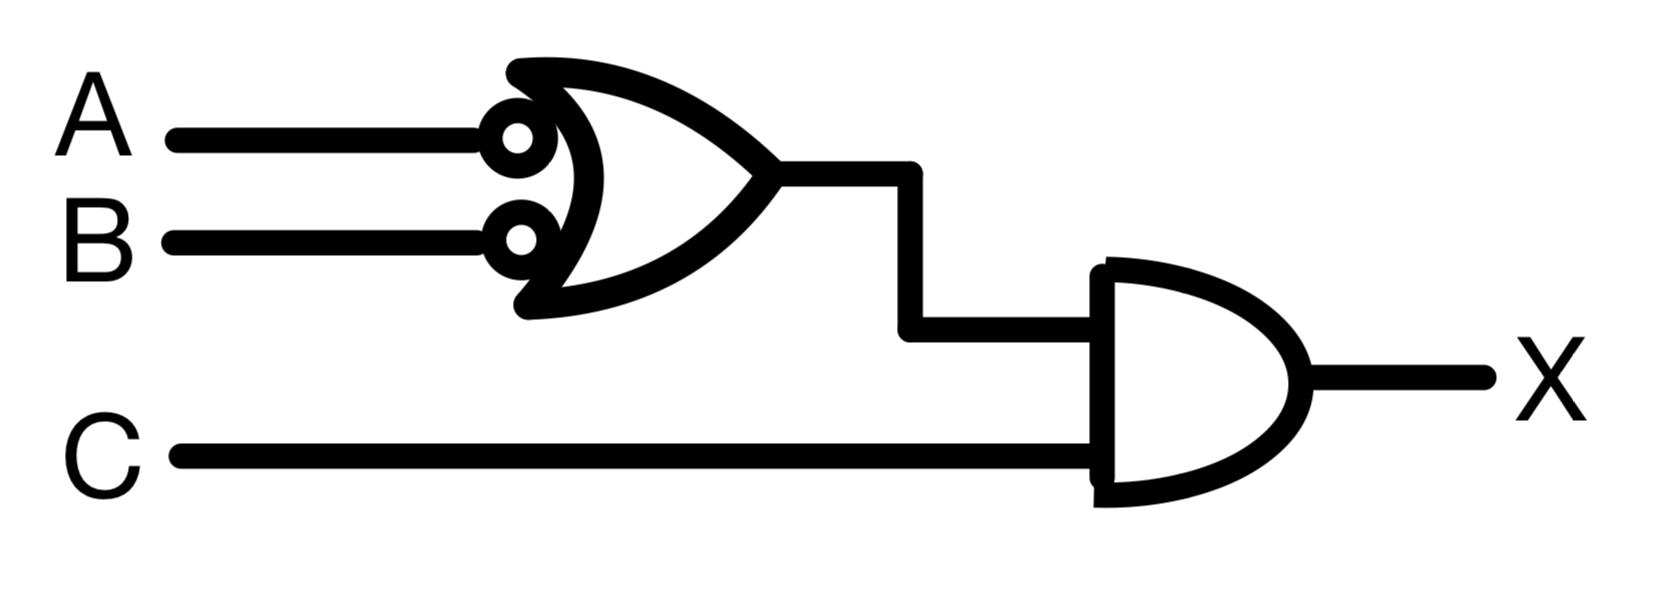
\includegraphics[scale=0.1]{figs/p1a.jpeg} \\
                $X = A(B' + C')$
            \end{center}

            Active low circuit:
            \begin{center} 
                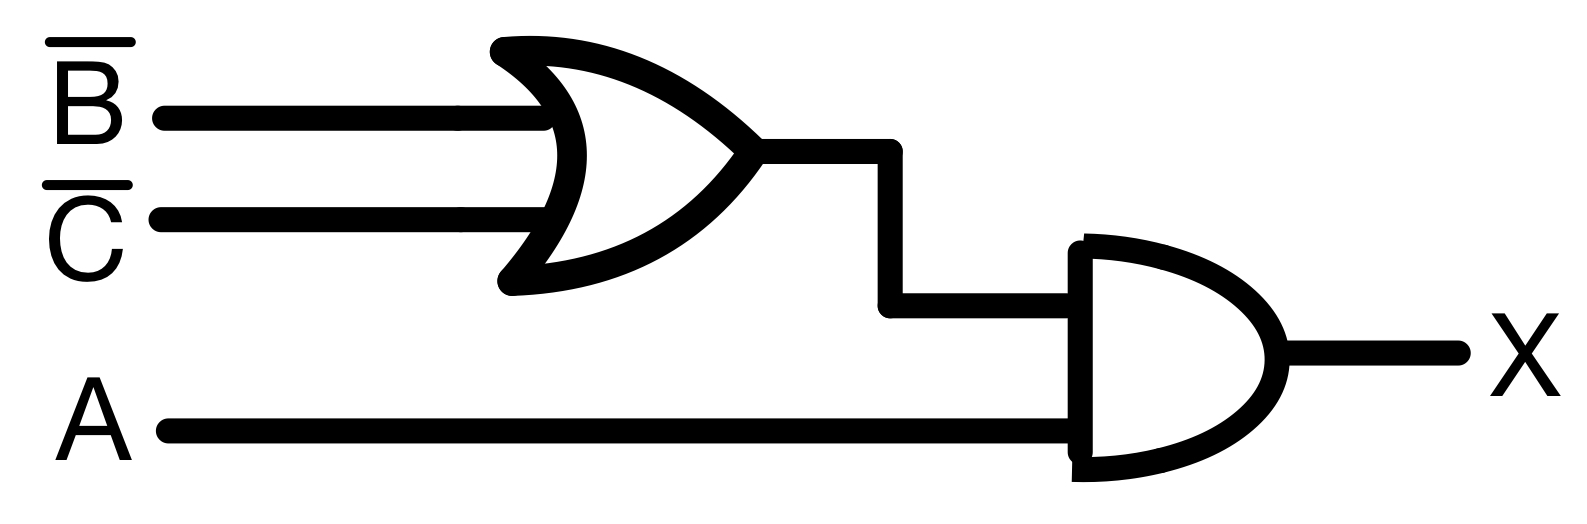
\includegraphics[scale=0.1]{figs/p1b.jpeg} \\
                $X = A(B' + C')$
            \end{center}

        \item \textbf{Problem 2}: \emph{Gray Code to Binary Converter} \\
            \begin{itemize}
                \item From inspection of the truth table, it is immediately
                apparent that $B_2 = G_2$. 

                \item For $B_1$, inspect the cases in which $G_2$ is active.
                There are 4 such cases: $(G_2, G_1, G_0) = \{(0, 1, 1),
                (0, 1, 0), (1, 0, 1), (1, 0, 0)\}$. It is clear that we may
                eliminate $G_0$ leaving the following: $(G_2, G_1) = {(0, 1),
                (1, 0)}$. This clearly shows $B_1 = G_2 \oplus G_1$

                \item For $B_0$, enumerate the active cases as an equation and
                simplify:
                \[B_0 = (G_2G_1'G_0')+(G_2'G_1'G_0)+(G_2G_1G_0)+(G_2'G_1G_0')\]
                \[B_0 = G_2(G_1'G_0' + G_1G_0)+G_2'(G_1'G_0+G_1G_0')\]
                \[B_0 = G_2(G_1 \oplus G_0)' + G_2'(G_1 \oplus G_0)\]
                \[B_0 = G_2 \oplus G_1 \oplus G_0\]

            \end{itemize}
            \begin{center}
                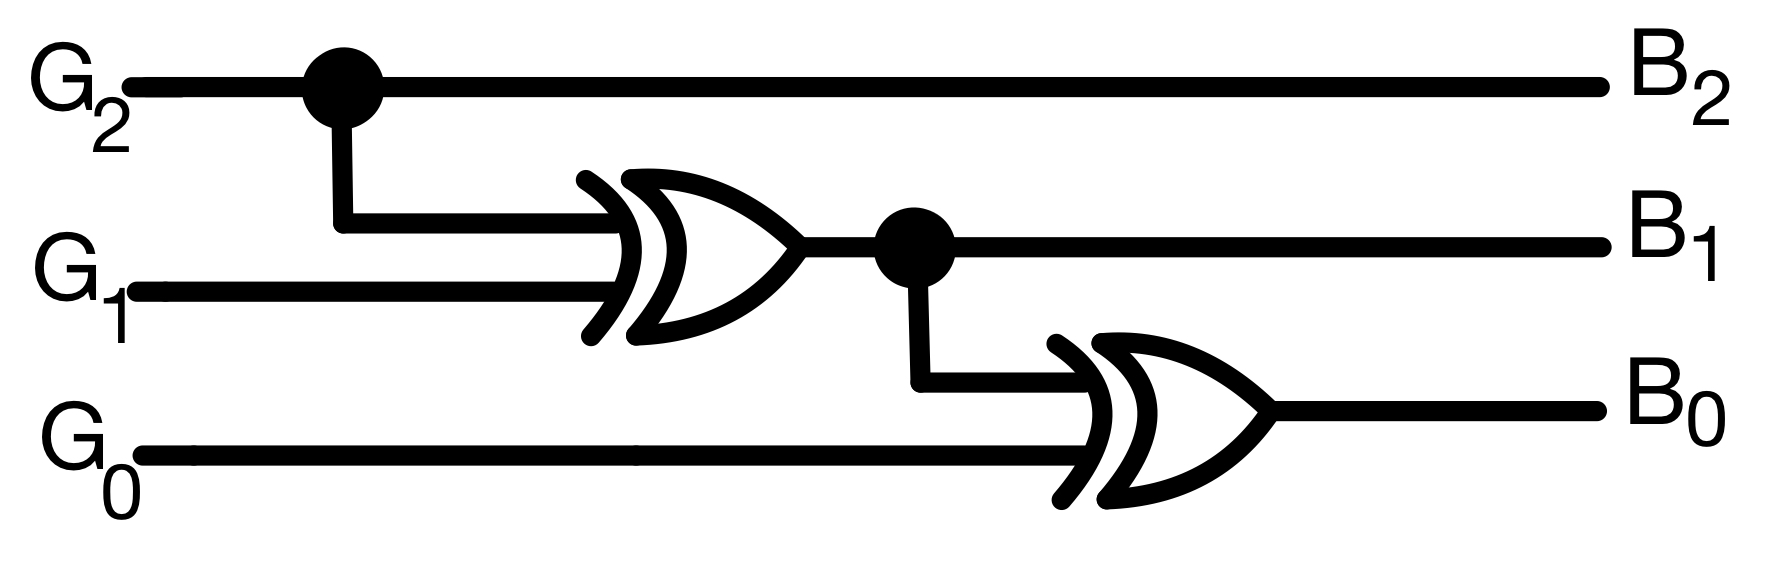
\includegraphics[scale=0.1]{figs/p2.jpeg}
            \end{center}

        \pagebreak
        \item \textbf{Problem 3}: \emph{Squaring Circuit} \\
        
        First, create the truth table for the circuit. Then consider
        the active cases for each output bit seperately.

        \begin{center}
            \begin{tabular} {|c c c c|c c c c c c c c|}
                \hline
                $B_3$ & $B_2$ & $B_1$ & $B_0$ & $S_7$ & $S_6$ & $S_5$ & $S_4$ & $S_3$ & $S_2$ & $S_1$ & $S_0$ \\
                \hline
                0&0&0&0&0&0&0&0&0&0&0&0 \\
                0&0&0&1&0&0&0&0&0&0&0&1 \\
                0&0&1&0&0&0&0&0&0&1&0&0 \\
                0&0&1&1&0&0&0&0&1&0&0&1 \\
                0&1&0&0&0&0&0&1&0&0&0&0 \\
                0&1&0&1&0&0&0&1&1&0&0&1 \\
                0&1&1&0&0&0&1&0&0&1&0&0 \\
                0&1&1&1&0&0&1&1&0&0&0&1 \\
                1&0&0&0&0&1&0&0&0&0&0&0 \\
                1&0&0&1&0&1&0&1&0&0&0&1 \\
                1&0&1&0&0&1&1&0&0&1&0&0 \\
                1&0&1&1&0&1&1&1&1&0&0&1 \\
                1&1&0&0&1&0&0&1&0&0&0&0 \\
                1&1&0&1&1&0&1&0&1&0&0&1 \\
                1&1&1&0&1&1&0&0&0&1&0&0 \\
                1&1&1&1&1&1&1&0&0&0&0&1 \\
                \hline
            \end{tabular}
        \end{center}

        \begin{itemize}
            \item For $S_0$ trivially notice from the truth table that \fbox{$S_0 = B_0$}
            \item For $S_1$, trivially notice that \fbox{$S_1 = 0$} always
            \item For $S_2$, the cases are 0010, 0110, 010, 1110. This holds all
            cases for $B_3$ and $B_2$ so that they can be eliminated, leaving
            \fbox{$S_2 = B_1B_0'$}
            \item For $S_3$, the cases are 0011, 0101, 1011, 1101. Clearly $B_0$
            must be active. $B_3$ may be eliminated, since its value makes no 
            difference. Notice that either $B_2$ or $B_1$ are always active but
            never both. Therefore, \fbox{$S_3 = B_0(B_2 \oplus B_1)$}.
            \item For $S_4$, the cases are 0100, 0101, 0111, 1001, 1011, 1100.
            Notice that for the cases where $B_0$ is active:
            \[S_4 = B_0B_3'B_2 + B_0B_3B_2'\]
            \[S_4 = B_0(B_3'B_2+B_3B_2')\]
            \[S_4 = B_0(B_3 \oplus B_2)\]
            This leaves 2 cases, 0100 and 1100. From these, $B_3$ is eliminated
            leaving $S_4 = B_0'B_1'B_2$. Therefore, \fbox{$S_4 =
            B_0(B_3 \oplus B_2) + B_0'B_1'B_2$}
            \item For $S_5$, the cases are 0110, 0111, 1010, 1011, 1101, 1111. 
            Eliminating trivial terms, these cases are summed up as follows:
            \[S_5 = B_1B_2B_3 + B_1B_2'B3 + B_0B_2B_3\]
            \[S_5 = B_1(B_2B_3'+B_2'B_3) + B_0B_2B_3\]
            Then \fbox{$S_5 = B_1(B_2 \oplus B_3) + B_0B_2B_3$}
            \item For $S_6$, the cases are 1000, 1001, 1010, 1011, 1110, 1111.
            Immediately notice that $B_3$ always must be active. When $B_0$ is 
            low, notice that $B_1$ and $B_0$ enumerate all cases and may be
            eliminated. This leaves only the cases where $B_2$ is active, in 
            which case $B_0$ enumerates all of its possibilities but all other 
            inputs are active. Combining all factors, \fbox{$S_6 = B_3(B_2'+B_2B_1)$}
            \item For $S_7$, the cases are the last 4 in the truth table. It is 
            obvious to see that these are the only 4 cases where both $B_3$ and
            $B_2$ are active. Therefore, \fbox{$S_7 = B_2B_3$}.
        \end{itemize}
        \begin{center}
            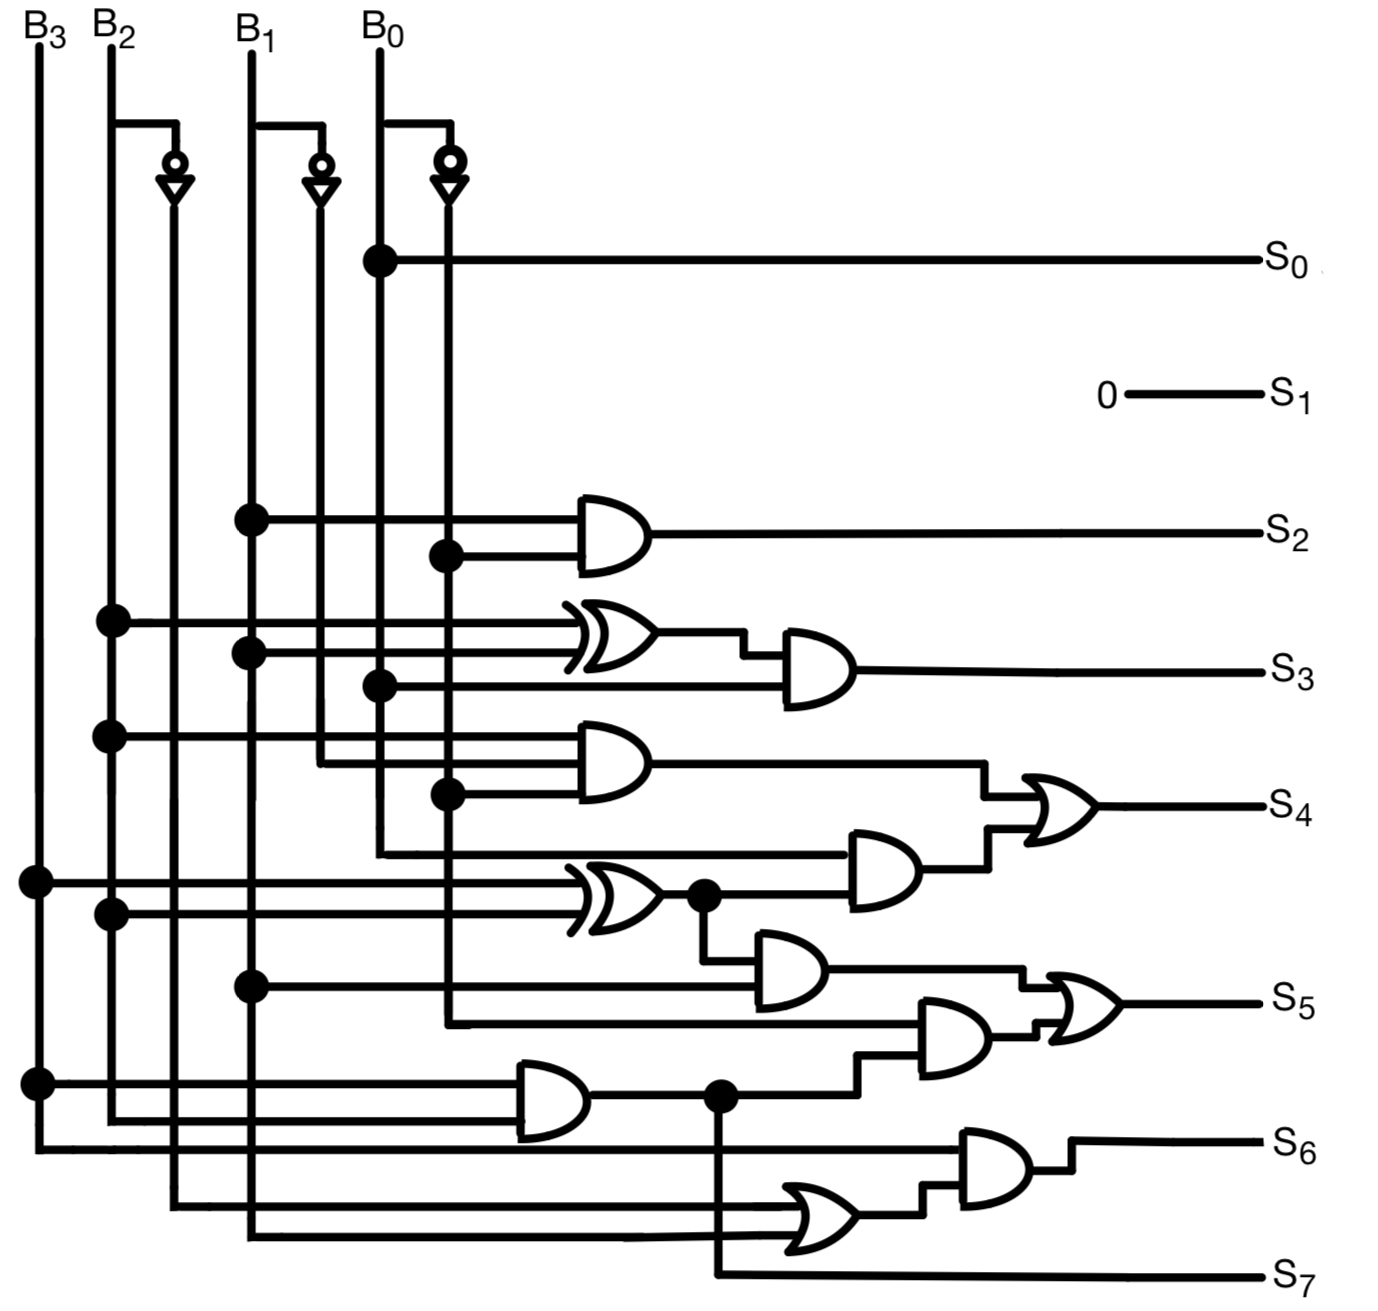
\includegraphics[scale=0.2]{figs/p3.jpeg}
        \end{center}

        \item \textbf{Problem 4}: \emph{Binary to BCD Hours Converter} \\
        
        Notice from the truth table that \fbox{$B_0 = Q_0$}, and that 
        \fbox{$B_2 = Q_2$}. Then solve for the remaining equations using
        Karnaugh maps.

        \begin{center}
            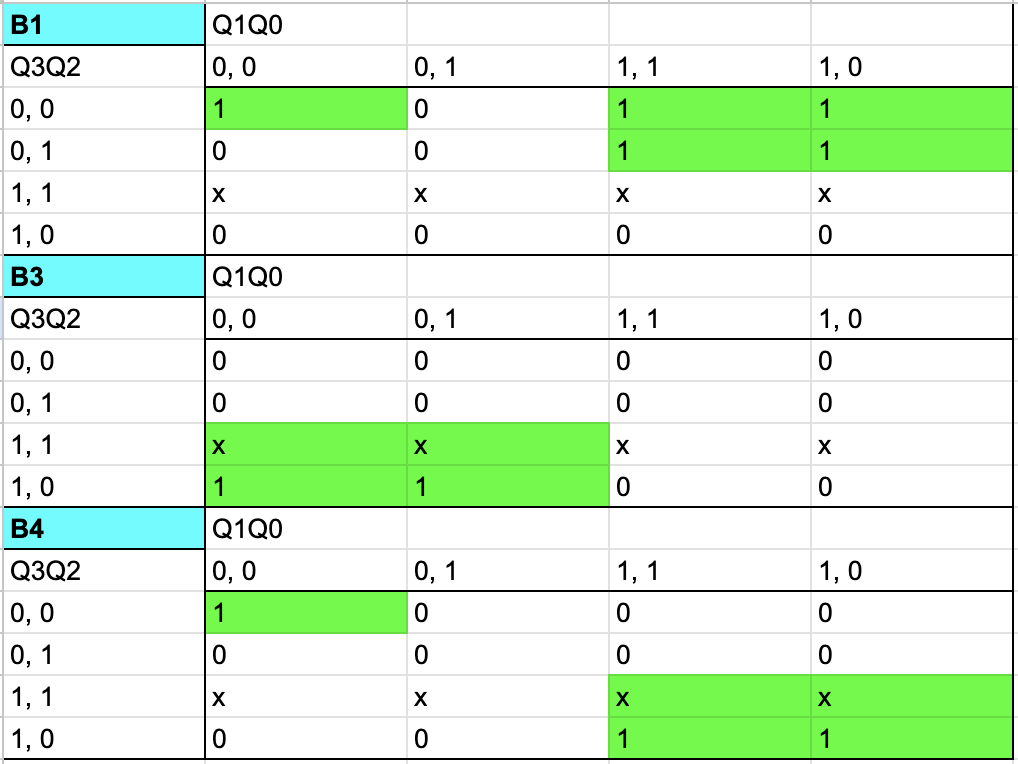
\includegraphics[scale=0.5]{figs/p4k.png}
        \end{center}

        These Karnaugh maps reveal the following:
        \begin{itemize}
            \item \fbox{$B_1 = Q_3'Q_1 + Q_3'Q_2'Q_0'$}
            \item \fbox{$B_3 = Q_3Q_1'$}
            \item \fbox{$B_4 = Q_3'Q_1 + Q_3'Q_2'Q_0'$}
        \end{itemize}

        AND/OR/INVERT circuit:
        \begin{center}
            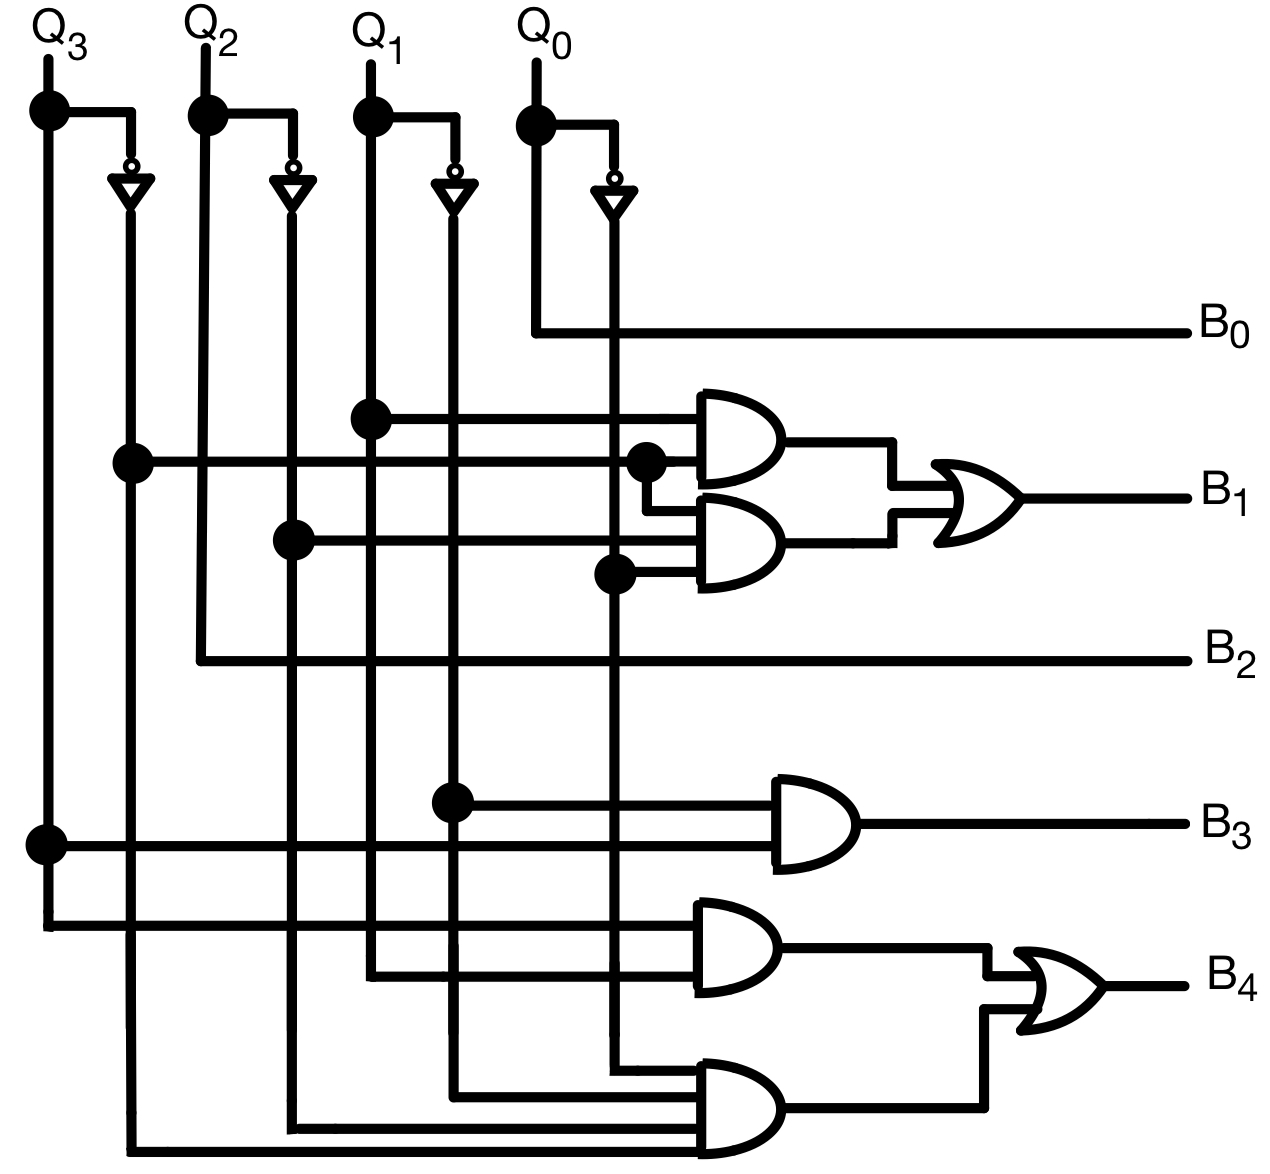
\includegraphics[scale=0.2]{figs/p4a.jpeg}
        \end{center}

        NAND/NAND circuit:
        \begin{center}
            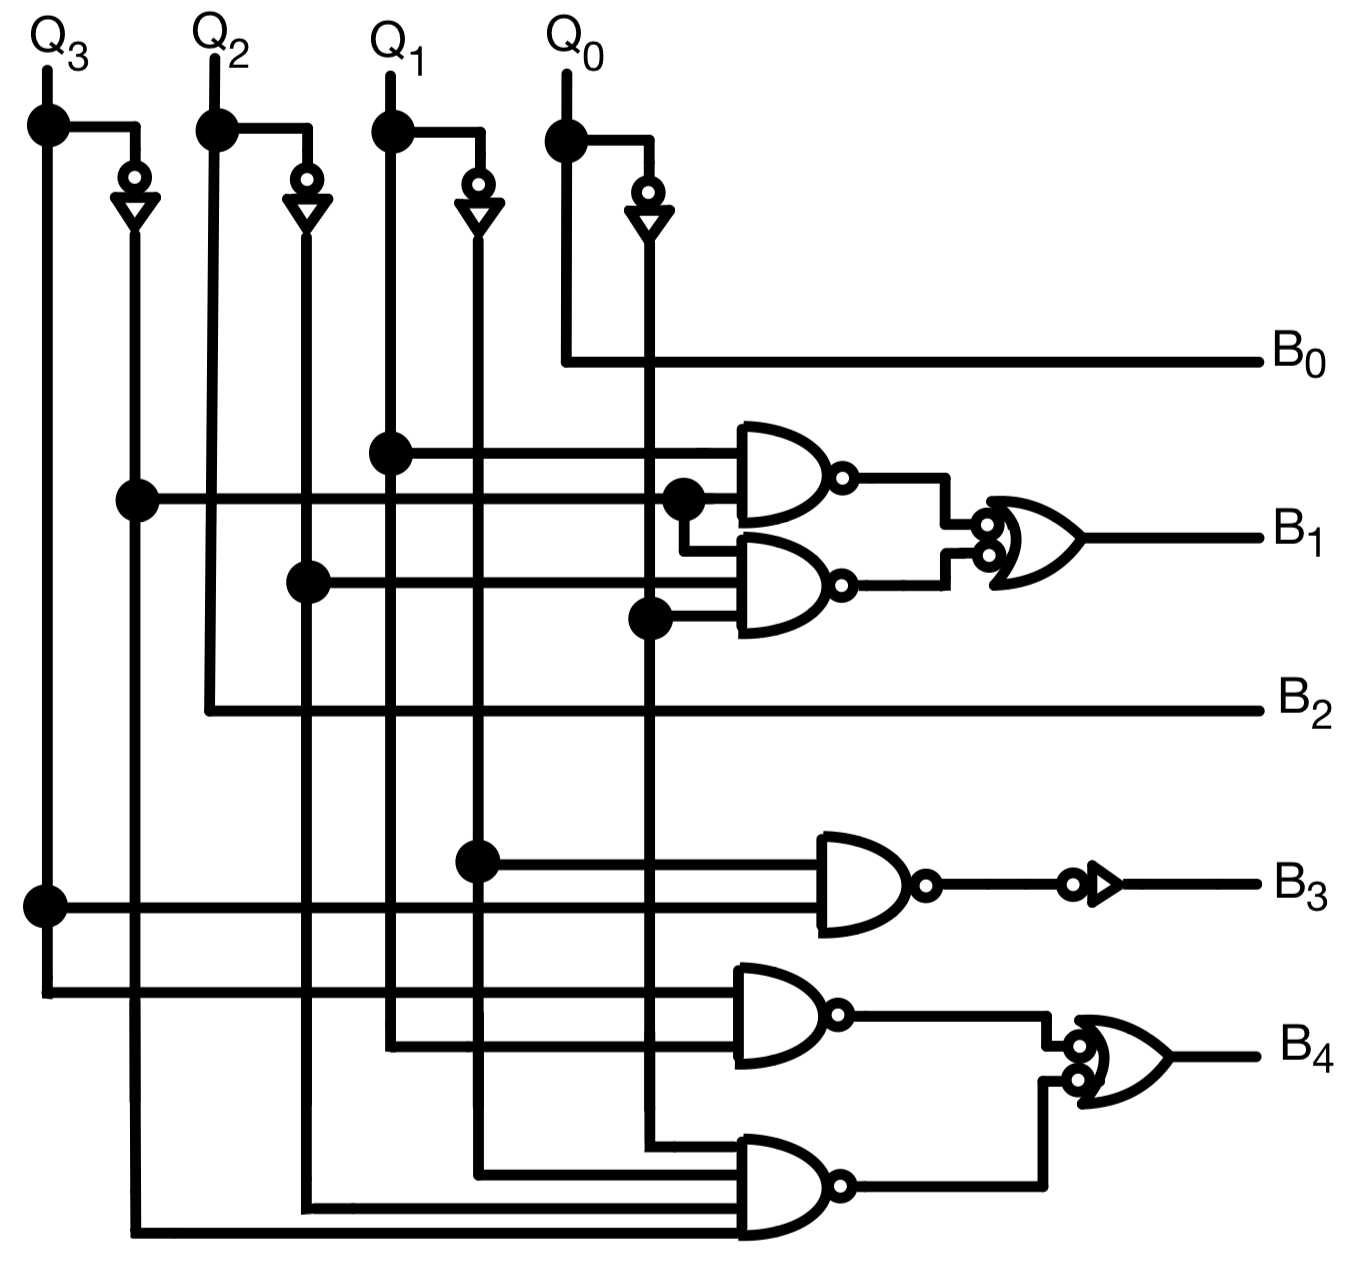
\includegraphics[scale=0.2]{figs/p4b.jpeg}
        \end{center}

    \end{enumerate}

\end{document}
